\section{Istruzioni d'uso}

\subsection{Cliente} % --------------------- SECTION DEL CLIENTE ---------------------%

\subsubsection{Accesso cliente}
Questa è la schermata di accesso per il cliente, dove gli utenti non autenticati possono inserire le proprie credenziali di accesso, costituite dall'\textit{email} e dalla {password}. 
Dopo aver compilato i campi, cliccando il pulsante "Accedi", gli utenti verranno reindirizzati alla propria pagina \textit{home} di pertinenza.

\begin{figure}[h]
    \centering
    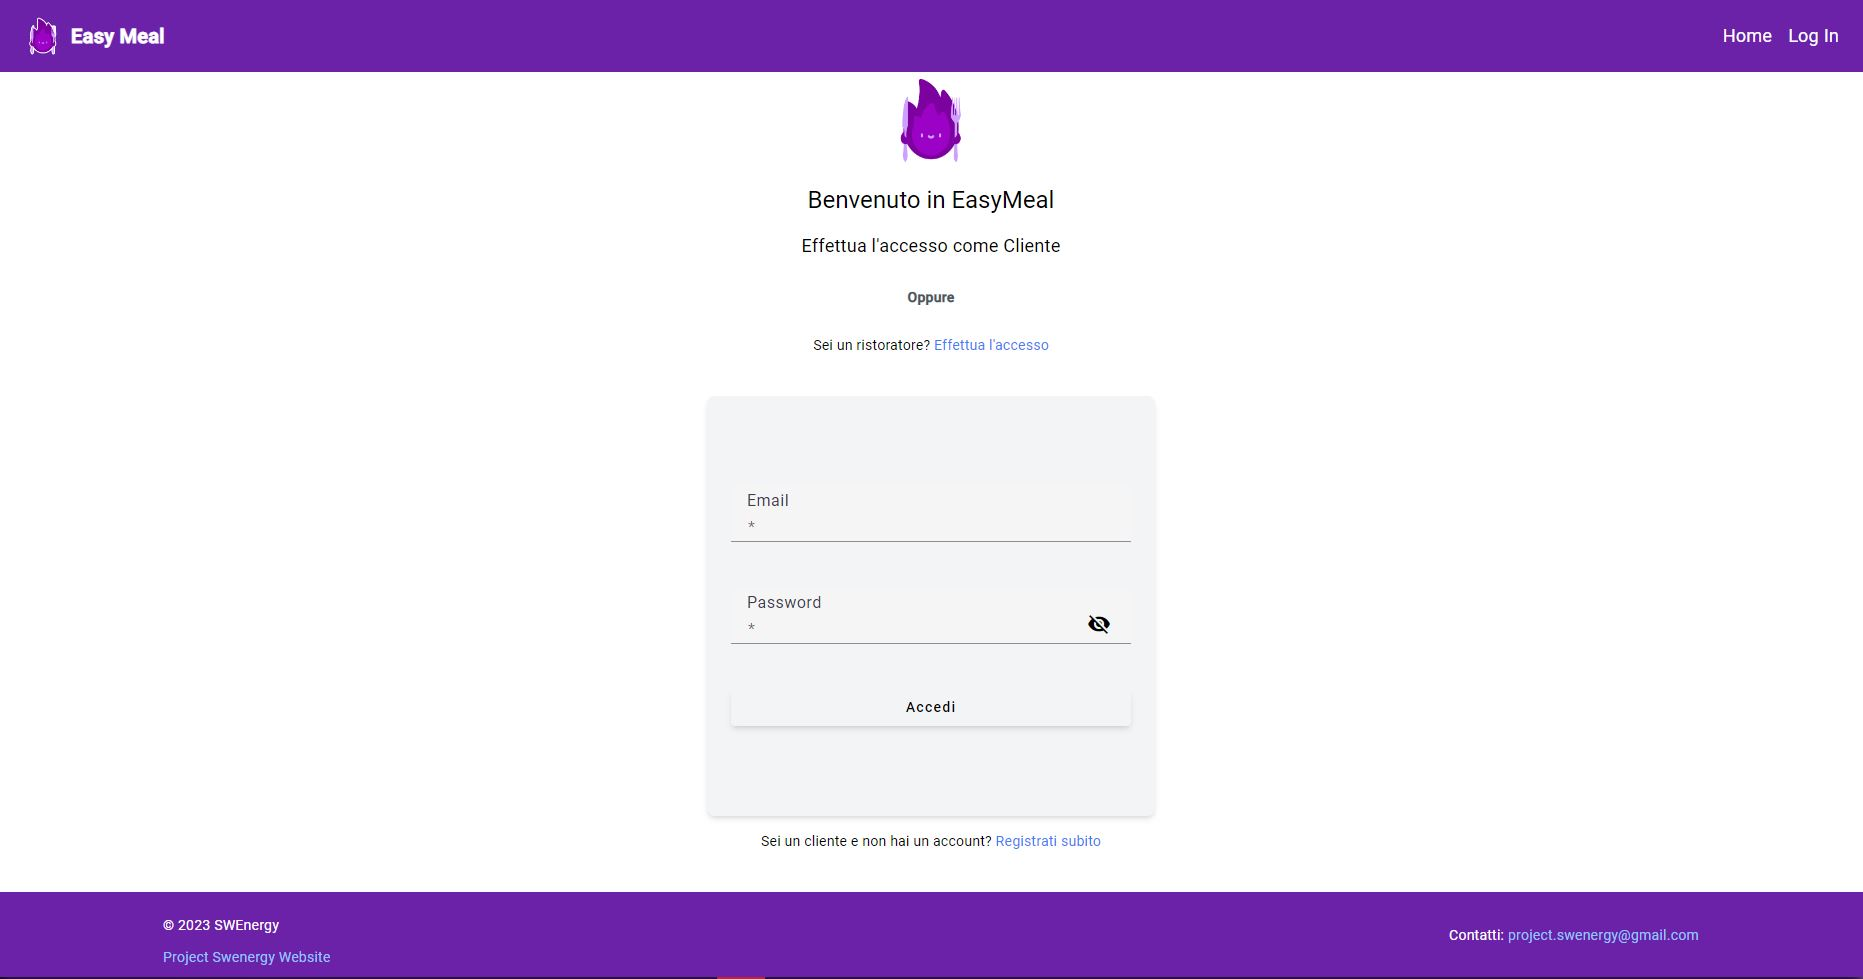
\includegraphics[width=0.9\textwidth]{./img/loginCliente.jpg}
    \caption{Pagina di login del cliente}
    \label{fig:esempio}
\end{figure}

Qui l'utente, nel caso non fosse registrato, può cliccare sul \textit{link} "Registrati subito" per essere reindirizzato alla pagina di registrazione del cliente.
Nel caso l'utente che stia visitando questa pagina non sia un cliente, bensì un ristoratore, può cliccare sul \textit{link} "Sei un ristoratore? Effettua l'accesso" 
per essere reindirizzato alla pagina di accesso del ristoratore.

\subsubsection{Permessi non corretti}
Se l'utente non fosse autenticato ad accedere ad una determina pagina, verrò reindirizzato alla seguente schermata:
IMMAGINE DA INSERIRE

\subsubsection{Pagina inesistente}
SE SI FA NEL MVP ALLORA VA MESSA + IMMAGINE, ALTRIMENTI SI CANCELLA QUELLO SCRITTO:
Si noti che se l'utente cerca di accedere ad una pagina che non esiste, verrà reindirizzato alla
seguente schermata, da cui in ogni momento potrà ritornare alla propria pagina principale.


\subsubsection{Registrazione cliente}
Questa è la schermata di registrazione per il cliente, dove gli utenti che non hanno un \textit{account} possono crearne uno.
Le informazioni da inserire per poter creare un profilo sono le seguenti:
\begin{itemize}
    \item Nome
    \item Cognome
    \item Email
    \item Password
    \item CONTINUARE AD AGGIUNGER IN CASO
\end{itemize}

\newpage
\begin{figure}[h]
    \centering
    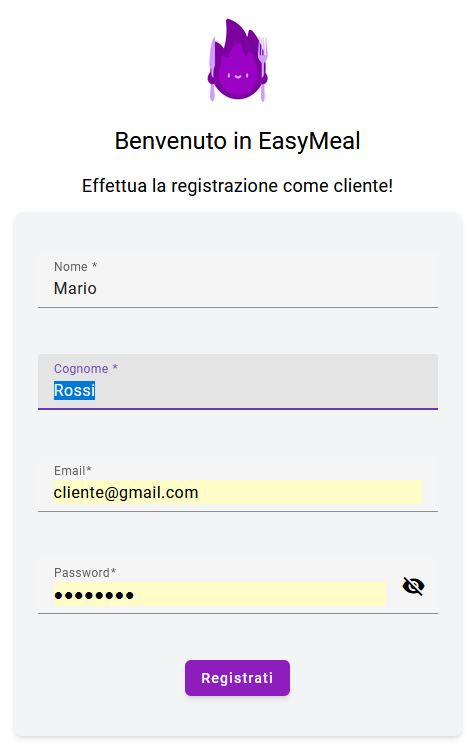
\includegraphics[width=0.9\textwidth]{./img/registrazioneCliente.jpg}
    \caption{Pagina di registrazione del cliente}
    \label{fig:esempio}
\end{figure}

Dopo aver compilato i campi, cliccando il pulsante "Registrati", gli utenti verranno reindirizzati alla propria pagina \textit{home} di pertinenza.



\subsection{Ristoratore} % --------------------- SECTION DEL RISTORATORE ---------------------%

\subsubsection{Accesso ristoratore}
Questa è la schermata di accesso per il ristoratore, dove gli utenti non autenticati possono inserire le proprie credenziali di accesso, costituite dall'\textit{email} e dalla {password}. 
Dopo aver compilato i campi, cliccando il pulsante "Accedi", gli utenti verranno reindirizzati alla propria pagina \textit{home} di pertinenza.

\newpage
\begin{figure}[h]
    \centering
    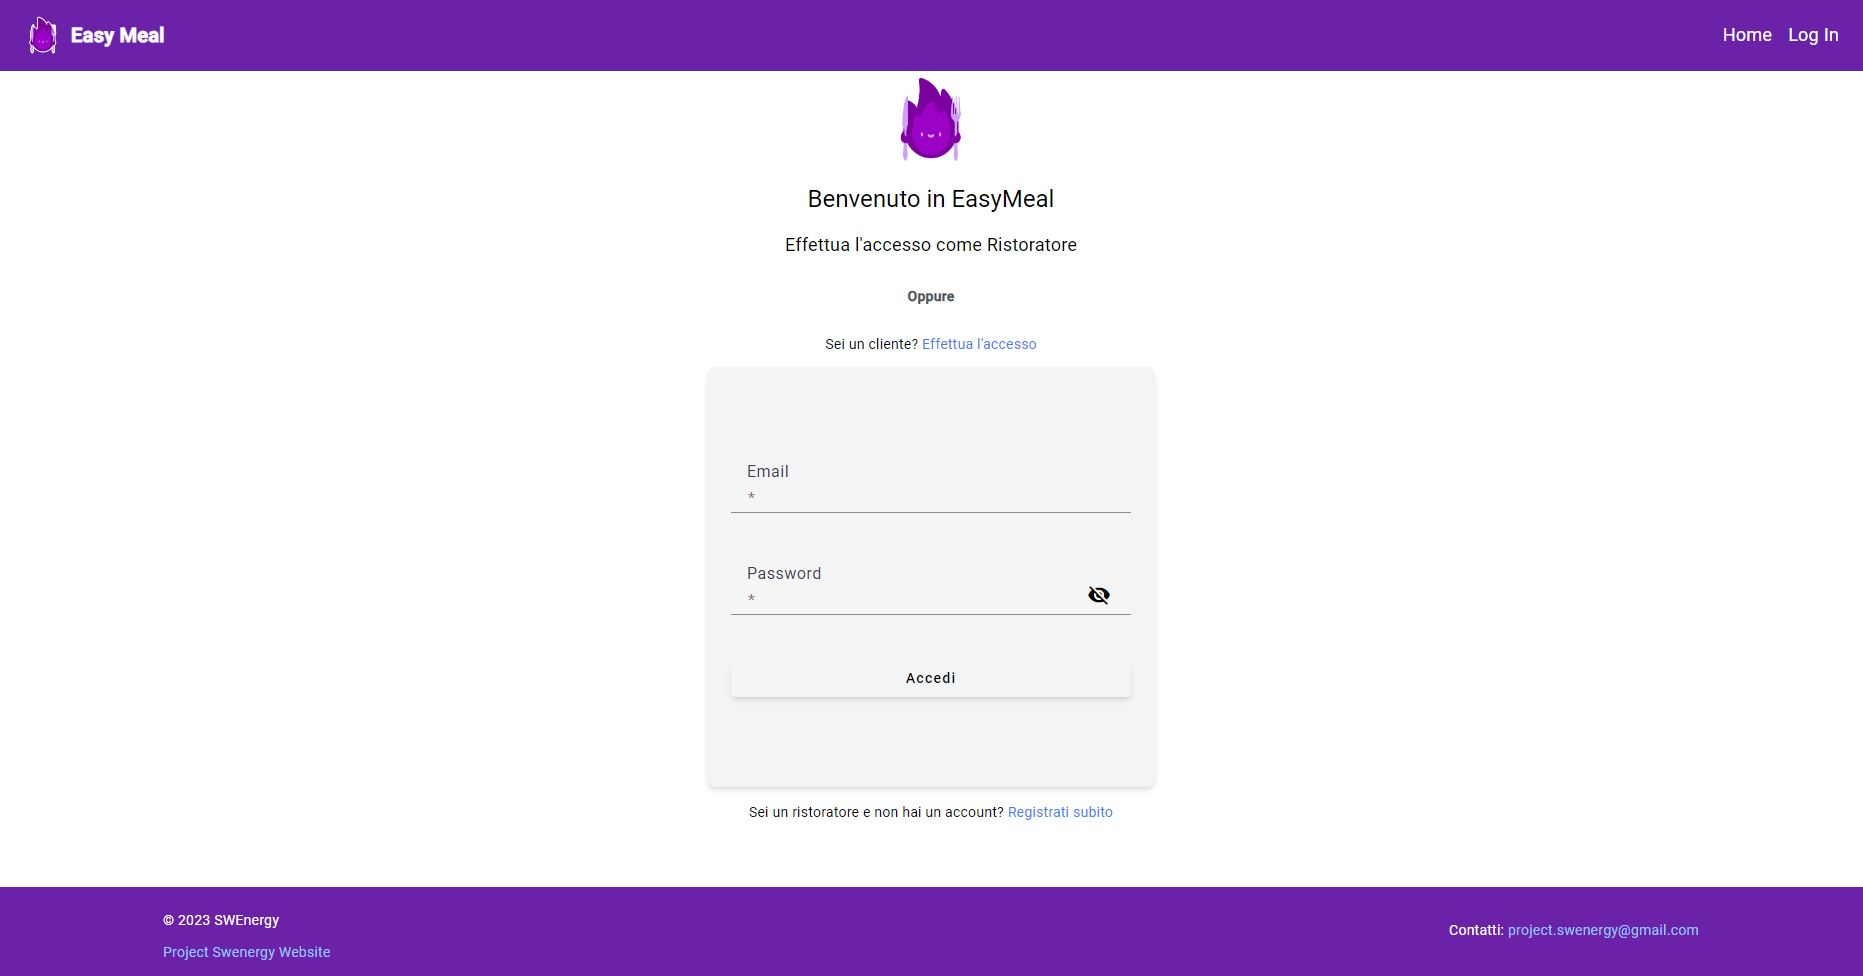
\includegraphics[width=0.9\textwidth]{./img/loginRistoratore.jpg}
    \caption{Pagina di login del ristoratore}
    \label{fig:esempio}
\end{figure}

Qui l'utente, nel caso non fosse registrato, può cliccare sul \textit{link} "Registrati subito" per essere reindirizzato alla pagina di registrazione del ristoratore.
Nel caso l'utente che stia visitando questa pagina non sia un ristoratore, bensì un cliente, può cliccare sul \textit{link} "Sei un cliente? Effettua l'accesso" 
per essere reindirizzato alla pagina di accesso del cliente.

\subsubsection{Permessi non corretti}
Se l'utente non fosse autenticato ad accedere ad una determina pagina, verrò reindirizzato alla seguente schermata:
IMMAGINE DA INSERIRE

\subsubsection{Pagina inesistente}
SE SI FA NEL MVP ALLORA VA MESSA + IMMAGINE, ALTRIMENTI SI CANCELLA QUELLO SCRITTO:
Si noti che se l'utente cerca di accedere ad una pagina che non esiste, verrà reindirizzato alla
seguente schermata, da cui in ogni momento potrà ritornare alla propria pagina principale.

\subsubsection{Registrazione ristoratore}
Questa è la schermata di registrazione per il ristoratore, dove gli utenti che non hanno un \textit{account} possono crearne uno.
Le informazioni da inserire per poter creare un profilo sono le seguenti:
\begin{itemize}
    \item Nome
    \item Cognome
    \item Email
    \item Password
    \item CONTINUARE AD AGGIUNGER IN CASO
\end{itemize}

\begin{figure}[h]
    \centering
    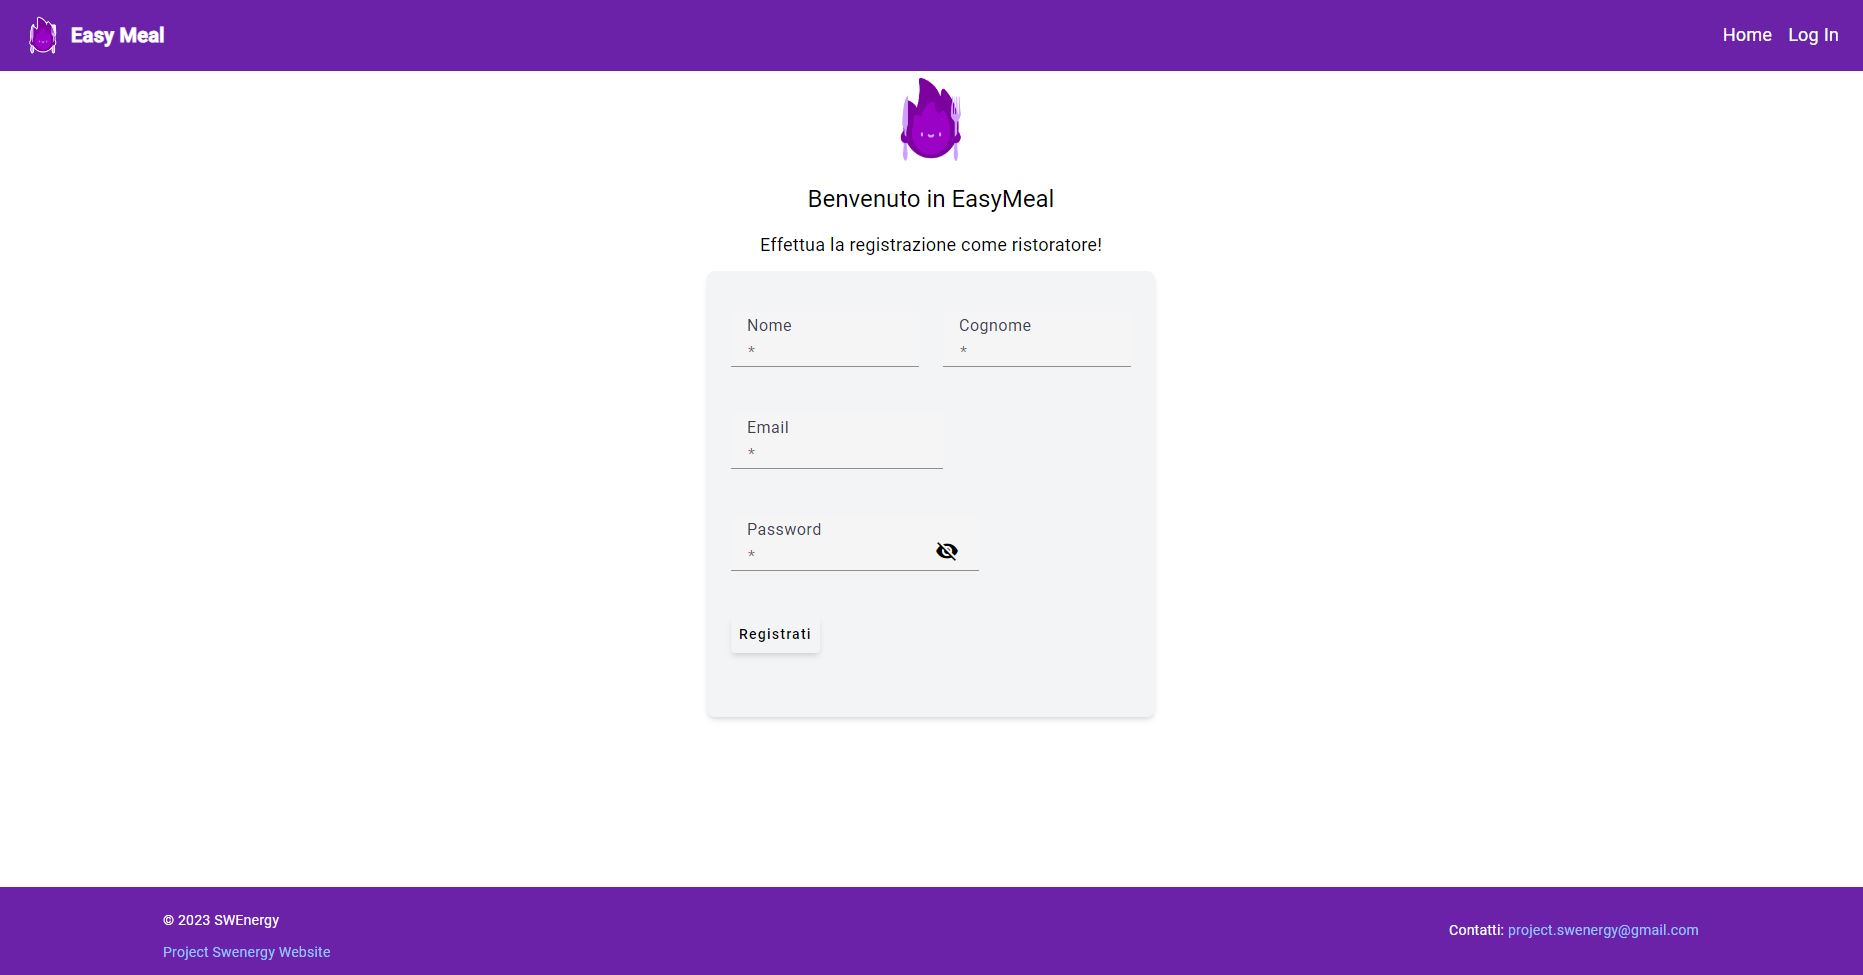
\includegraphics[width=0.9\textwidth]{./img/registrazioneRistoratore.jpg}
    \caption{Pagina di registrazione del ristoratore}
    \label{fig:esempio}
\end{figure}

Dopo aver compilato i campi, cliccando il pulsante "Registrati", gli utenti verranno reindirizzati alla propria pagina \textit{home} di pertinenza.
